\documentclass[8pt]{beamer}

\usepackage[utf8]{inputenc}
\usepackage[T1]{fontenc}
\usepackage[francais]{babel}

\usepackage{longtable}
\usepackage{booktabs}
\usepackage{multirow}

\usepackage{graphicx}
\usepackage{subcaption}
\usepackage{floatrow}
\captionsetup{labelsep=period}

\usepackage[]{algorithm2e}
\SetKwRepeat{Do}{do}{while}

\usepackage{standalone}

\usepackage{amssymb, amsmath, mathrsfs, mathtools, dsfont, bbold, cancel}

\usetheme{ign}

\title{Classification et apprentissage statistique}
\subtitle{Supervisé et non-supervisé}
\author{Oussama ENNAFII}
\institute{ENSG}
\date{\today}

\begin{document}

	\begin{frame}[plain]
		\titlepage{}
	\end{frame}

	\section{Introduction}
		\begin{frame}{Classification: première définition}
			Champs lexical de classer :
			\begin{itemize}
				\item<2-> ranger,
				\item<3-> labeliser,
				\item<4-> catégoriser,
				\item<5-> hiérarchiser.
			\end{itemize}
			\uncover<6->{
				\begin{block}{Esquisse de définition}
					Classer: ranger \(n\) \textbf{objets} dans \(k\) \textbf{catégories} (avec \(k \ll n\)).
				\end{block}
			}
		\end{frame}
		
		\begin{frame}{Comment classer?}
			\begin{itemize}
					\item<1-> Comment caractériser un objet à classer ?
					\item<2-> Comment sont définies les catégories (ou classes) d'objets?
			\end{itemize}
		\end{frame}
	
	\section{Classification}
		\subsection{Exemples}
			\begin{frame}{Reconaissance d'objet}
				\begin{figure}[H]
					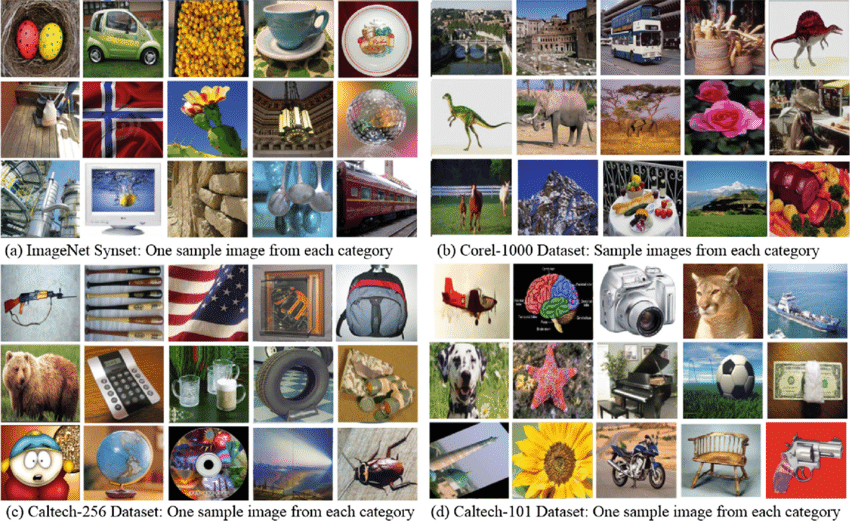
\includegraphics[width=.7\textwidth]{images/samples/image_datasets}
					\caption*{\tiny Exemples de base de données d'images~\cite{ahmed2017fusion}.}
				\end{figure}
			\end{frame}
			
			\begin{frame}{Occupation du sol}
				\begin{figure}[H]
					\ffigbox[\FBwidth]
					{
						\begin{subfloatrow}[2]
							\ffigbox[\FBwidth]
							{
								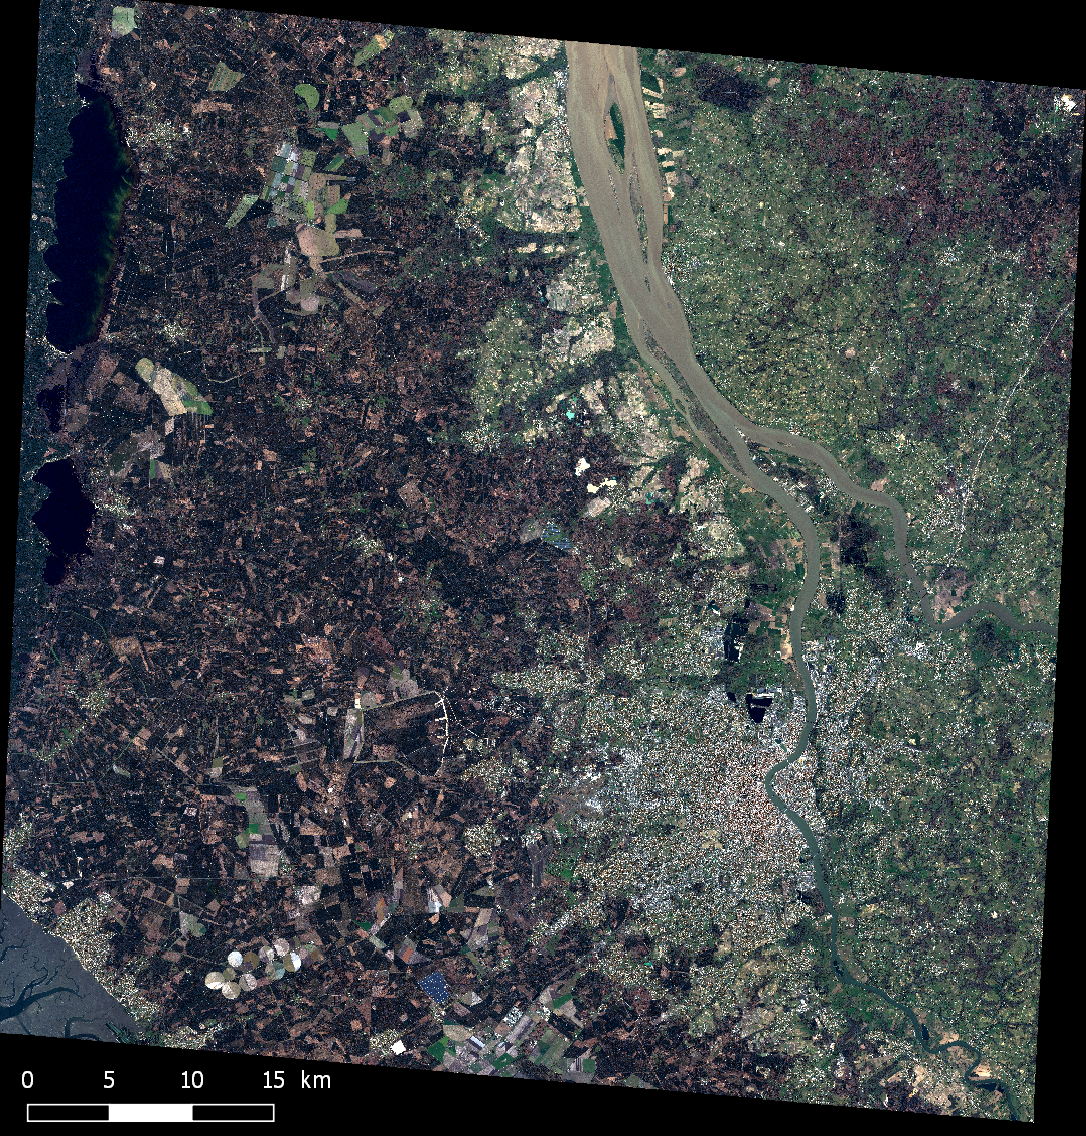
\includegraphics[width=.31\textwidth]{images/samples/gironde}
							}
							{
								\caption*{\tiny Image de la Gironde prise par SPOT en 2016: Résolution 1.5m, 4 canaux: \{{\color{purple!20}Infrarouge}, {\color{red}Rouge}, {\color{green}Vert}, {\color{blue}Bleu}\}.}
							}
							\ffigbox[\FBwidth]
							{
								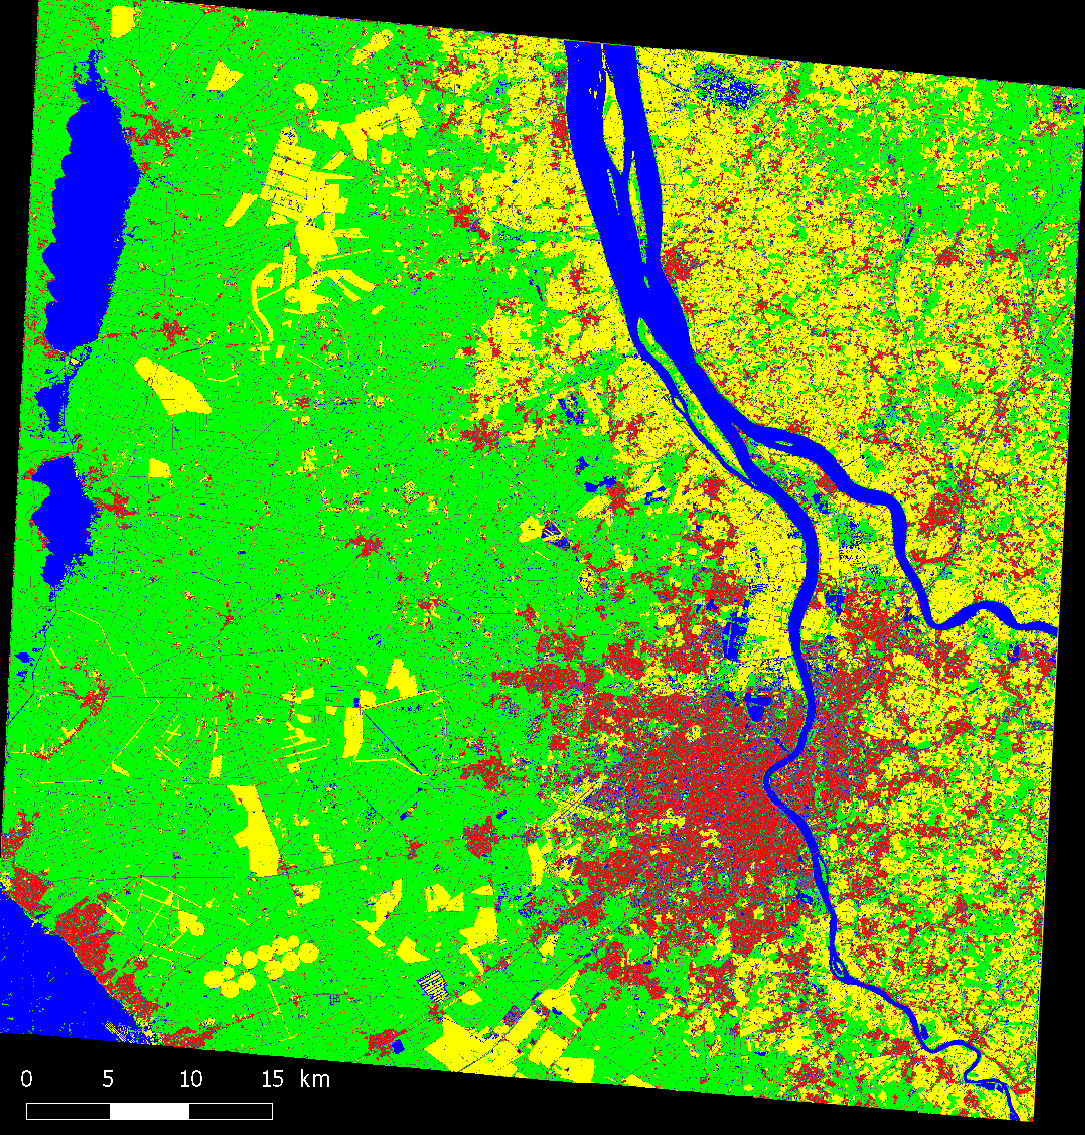
\includegraphics[width=.31\textwidth]{images/samples/gironde_classif}
							}
							{
								\caption*{\tiny Occupation des sols extraite de l'image: {\color{red}\(\blacksquare\)} Bâti, {\color{green}\(\blacksquare\)} Forêt, {\color{yellow}\(\blacksquare\)} Culture, {\color{gray}\(\blacksquare\)} Routes, {\color{blue}\(\blacksquare\)} Eau.}
							}
						\end{subfloatrow}
					}
					{
						\caption*{\tiny Classification appliquée pour l'Occupation des sols~\cite{postadjian2017investigating}.}
					}
				\end{figure}
			\end{frame}

			\begin{frame}{Segmentation de nuage de points}
				\begin{figure}[H]
					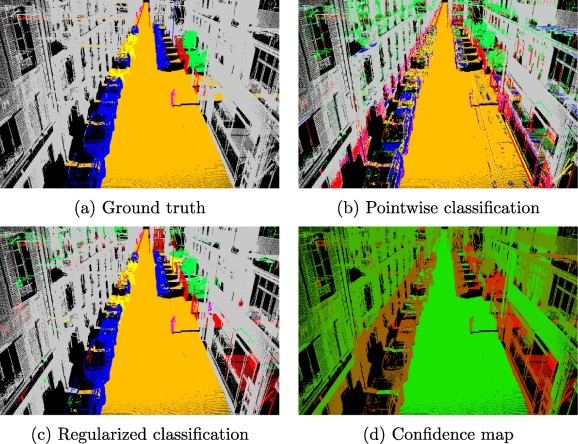
\includegraphics[width=.6\textwidth]{images/samples/pc_classification}
					\caption*{\tiny Exemple de classification de nuage de point\cite{landrieu2017structured}.}
				\end{figure}
			\end{frame}

			\begin{frame}{Détection de phénomènes}
				\begin{figure}[H]
					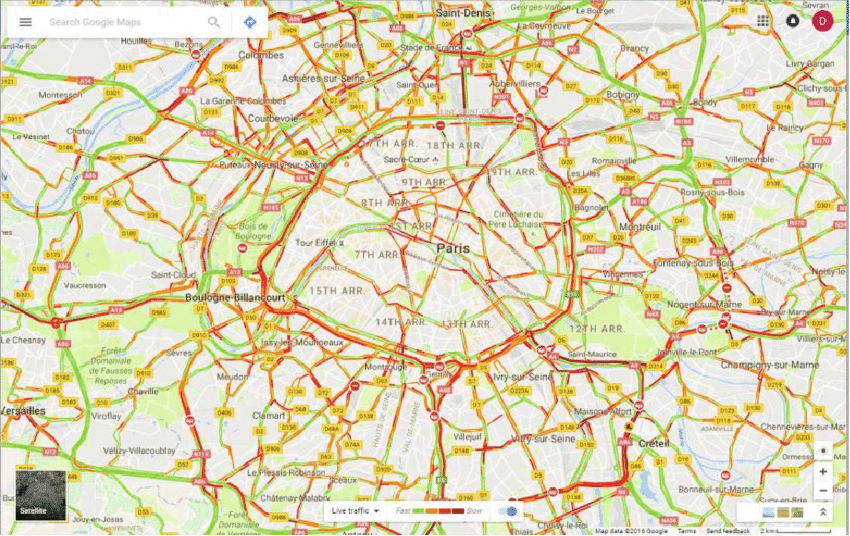
\includegraphics[width=.65\textwidth]{images/samples/traffic_paris}
					\caption*{\tiny Exemple de classification utilisé pour déterminer les conditions de circulation à Paris le 06/09/2016 à 9:30~\cite{tutic2016google}.}
				\end{figure}
			\end{frame}

			\begin{frame}{Classification avec RADAR}
				\begin{figure}[H]
					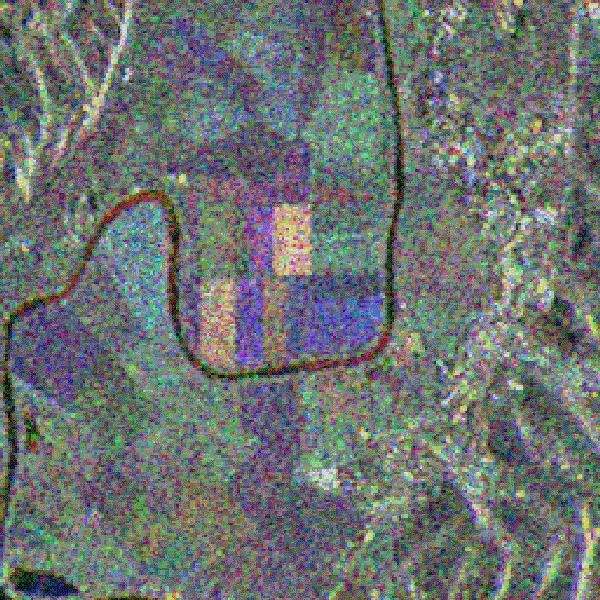
\includegraphics[width=.45\textwidth]{images/samples/radar}
					\caption*{\tiny Exemple d'occupation de sol utilisant basée RADAR~\cite{EsaRadar}.}
				\end{figure}
			\end{frame}

		\subsection{Observations}
			\begin{frame}{Comment caractériser les observations?}
				\begin{itemize}
					\item<1-> Comment sont représentées les données à classer?
					\item<2-> Quel est le point commun entre ces observations?
				\end{itemize}
			\end{frame}
		
			\begin{frame}{Observations}
				Les observations peuvent prendre beaucoup de formes:
				\begin{itemize}
					\item<2-> Image;
					\item<3-> Série temporelle (son, vidéo \dots);
					\item<4-> Graphe de données;
					\item<5-> Nuage de points (LiDAR par exemple).
				\end{itemize}
			\end{frame}

			\begin{frame}{Attributs: représentation vectorielle}
				\begin{itemize}
					\item<1-> On représente généralement les observables par un vecteur dans \(\mathbb{R}^d\) qu'on nome attributs.
					\item<2-> On notera la \(i\)-ème observation par \(X^i = \begin{pmatrix}
						X^i_1\\
						X^i_2\\
						\vdots\\
						X^i_d
					\end{pmatrix}\).
					\item<3-> On notera donc l'ensemble des observations par \(\big( X^i \big)_{i=1,\dots, n}\).
				\end{itemize}
			\end{frame}

		\subsection{Types d'apprentissage}
			\begin{frame}{Apprentissage: supervisé et non-supervisé}
				Les classes peuvent être:
				\begin{itemize}
					\item<2-> non définies \(\longrightarrow\) apprentissage non-supervisé;
					\item<3-> définies \(\longrightarrow\) apprentissage (ou classification) supervisé.
				\end{itemize}
			\end{frame}

	\section{Algorithmes non-supervisés}
		\subsection{Définition}
			\begin{frame}{Apprentissage non-supervisé}
				\begin{itemize}
					\item<1-> Dans le cas de l'apprentissage non-supervisé, on n'observe que les objets à classer, représentés par leurs attributs \(\big(X^i\big)_{i=1,\dots, n}\);
					\item<2-> Le but est de partitionner les instances homogènes se ``ressemblant'' en un seul cluster;
					\item<3-> La ressemblance est basée sur la distance entre deux objets dans l'espace des attributs;
					\item<4-> La partition guarantie:
						\begin{itemize}
							\item<5-> des distances faibles intra-cluster;
							\item<6-> des distances grandes inter-cluster.
						\end{itemize}
				\end{itemize}
			\end{frame}

			\begin{frame}{Apprentissage non-supervisé}
				\begin{figure}[H]
					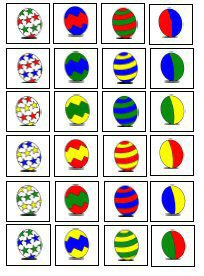
\includegraphics[height=.6\textheight]{images/samples/easter_non_supervised}
					\caption*{Exemple de problématique d'apprentissage non-supervisé.}
				\end{figure}
			\end{frame}

			\begin{frame}{Apprentissage supervisé}
				Comment choisir ses attributs pour représenter chaque observation sous forme de vecteur?
				\begin{itemize}
					\item<2-> nombre de côté du motif régulier;
					\item<3-> couleur rouge;
					\item<4-> couleur verte;
					\item<5-> couleur blanche;
					\item<6-> couleur bleue;
					\item<7-> couleur jaune;
					\item<8-> couleur orange;
					\item<9-> convexité du motif;
					\item<10-> symétrie par rotation du motif;
					\item<11-> symétrie par translation du motif;
					\item<12-> \dots;
				\end{itemize}
				\uncover<13->{
					Pour l'instance en haut à droite, le vecteur d'attributs s'écrit:
					\[\begin{pmatrix}
						5 & 1 & 1 & 1 & 0 & 0 & 0 & False & False & False \dots
					\end{pmatrix}^T\]
				}
			\end{frame}
			\begin{frame}{Apprentissage non-supervisé}
				\begin{figure}[H]
					\begin{center}
						\includestandalone[mode=buildnew, height=.5\textheight]{scatter_circles}
						\caption*{\tiny Exemple de problème non-supervisé: 2 attributs. Les classes ne sont pas données mais une structure se dégage.}
					\end{center}
				\end{figure}
			\end{frame}
			\begin{frame}{Apprentissage non-supervisé}
				\begin{figure}[H]
					\begin{center}
						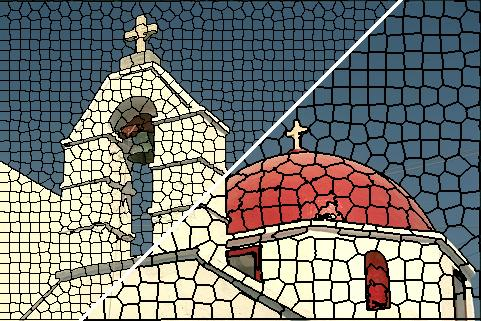
\includegraphics[height=.5\textheight]{images/samples/superpixels}
						\caption*{\tiny Exemple de problème non-supervisé: super-pixelisation d'une image~\cite{achanta2012slic}.}
					\end{center}
				\end{figure}
			\end{frame}

		\subsection{L'inertie}
			\begin{frame}{Variance intraclasse}
				\begin{itemize}
					\item<1-> Soit \(\big(S_k\big)_{k = 1, \dots, K}\) une \(K\)-partition de \(\{1, 2, \dots, n\}\).
					\item<2-> Pour chaque sous-ensemble \(S_k\), on définit la quantité
						\begin{equation}
							\sum_{i\in S_k} d(X^i, \mu_k)^2
						\end{equation}
					 où:
						\begin{itemize}
							\item<3-> \(d: \mathbb{R}^d \times \mathbb{R}^d \rightarrow \mathbb{R}_+\) représente une distance: dans tout ce qui suit \(d(x, y) = \lVert x - y \rVert\);
							\item<3-> \(\mu_k\) est le barycentre de \(S_k\): \( \mu_k \triangleq \frac{1}{\vert S_k \vert}.\sum_{i\in S_k} X^i\).
						\end{itemize}
					\item<4-> Cette quantité exprime la ``variance intraclasse'' de l'ensemble \(S_k\).
				\end{itemize}
			\end{frame}
			\begin{frame}{Pourquoi le nom ``variance intraclasse''?}
				\begin{itemize}
					\item<1-> Soit \(Z: \Omega \rightarrow \mathbb{R}^d\) une variable aléatoire telle que \(\mathbb{E}(Z) < \infty\) et \(\mathbb{E}(\lVert Z \rVert^2) < \infty\).
					\item<2-> Soient \(\big(Z^i\big)_{i=1,\dots,p}\) \(p\) réalisations indépendentes et identiquement distribuées (i.i.d) de même loi que \(Z\).
					\item<3-> Par définition, la variance empirique de \(\big(Z^i\big)_{i=1,\dots,p}\) est:
						\begin{equation}
							\text{Var}_{emp}(\big(Z^i\big)_{i=1,\dots,p}) \triangleq \frac{1}{p} . \sum_{i=1}^{p} \lVert Z^i - \bar Z \rVert^2 \underset{p\infty}{\longrightarrow} \text{Var}(Z) = \mathbb{E}(\lVert Z - \mathbb{E}(Z) \rVert^2)
						\end{equation}
						où \(\bar Z := \frac{1}{p}.\sum_{i=1}^{p} Z^i \underset{p\infty}{\longrightarrow} \mathbb{E}(Z)\).
					\item<4-> On considère les instances dans \(S_k\) comme réalisations d'une même loi de probabilité \(X_k\). On vérifie que:
						\begin{equation}
							V(S_k) = \sum_{i\in S_k} \lVert X^i - \mu_k \rVert^2 = \vert S_k \vert . \text{Var}_{emp}(X_k)
						\end{equation}
						On voit bien que cette quantité est liée à la variance des instances qui appartient au cluster \(S_k\).
				\end{itemize}
			\end{frame}
			\begin{frame}{Variance intraclasse: mesure d'hétérogéniété}
				\begin{itemize}
					\item<1-> On remarque aussi que:
						\only<1>{
							\scriptsize
							\begin{align*}
								\sum_{i,j\in S_k} \lVert X^i - X^j \rVert^2 &= \sum_{i,j\in S_k} \lVert (X^i -\mu_k) + (\mu_k - X^j) \rVert^2\\
																			&= \sum_{i,j\in S_k} \lVert X^i -\mu_k \rVert^2 + \lVert \mu_k - X^j \rVert^2 + 2 . \langle X^i -\mu_k , \mu_k - X^j \rangle\\
																			&= \sum_{i,j\in S_k} \lVert X^i -\mu_k \rVert^2 + \sum_{i,j\in S_k} \lVert \mu_k - X^j \rVert^2 + 2. \sum_{i,j\in S_k} \langle X^i -\mu_k , \mu_k - X^j \rangle\\
																			&= \vert S_k \vert . \sum_{i\in S_k} \lVert X^i -\mu_k \rVert^2 + \vert S_k \vert . \sum_{j\in S_k} \lVert X^j -\mu_k \rVert^2 + 2 . \langle \sum_{i\in S_k}(X^i -\mu_k) , \sum_{j\in S_k} (\mu_k - X^j) \rangle\\
																			&= 2. \vert S_k \vert . \sum_{i\in S_k} \lVert X^i -\mu_k \rVert^2 + 2.\langle \cancelto{0}{\sum_{i\in S_k} X^i - \vert S_k \vert.\mu_k}, \cancelto{0}{\vert S_k \vert.\mu_k - \sum_{j\in S_k} X^j}\rangle\\
																			&= 2. \vert S_k \vert . \sum_{i\in S_k} \lVert X^i -\mu_k \rVert^2
							\end{align*}
						}
						\uncover<2->{
							\begin{equation}
								\sum_{i,j\in S_k} \lVert X^i - X^j \rVert^2 = 2. \vert S_k \vert . \sum_{i\in S_k} \lVert X^i -\mu_k \rVert^2
							\end{equation}
						}
					\item<3-> Cette équation lie, proportionellement, le premier terme décrivant l'hétérogénéité de l'ensemble \(S_k\) avec le deuxième qui exprime la variance intraclasse.
					\item<4-> Le premier terme implique \(\frac{\vert S_k \vert.(\vert S_k \vert - 1)}{2}\) comparaisons alors que la variance intraclasse demande \(\big(\overbrace{\vert S_k \vert + 1}^{calcul\ de\ la\ moyenne}\big) + \big(\overbrace{\vert S_k \vert}^{comparaisons}\big)\).
					\item<5-> Calculer la variance intraclasse est plus efficace que de calculer la disparité de couples deux à deux, tout en exprimant la même information.
				\end{itemize}
			\end{frame}

			\begin{frame}{Inertie intraclasse}
				\begin{itemize}
					\item<1-> On somme les différentes disparités intra-cluster sur tout les sous-ensembles \(S_k\). On définit l'inertie intraclasse de la partition:
						\begin{equation}
							I_W(\big(S_k\big)_{k = 1, \dots, K}) \triangleq \sum_{k= 1}^{K} \sum_{i\in S_k} d(X^i, \mu_k)^2
						\end{equation}
					\item<2-> Pour le cas particulier de \(A=1\), on vérifie \(\big(S_k\big)_{k = 1} = (\{1,\dots,n\})\). On définit donc l'inertie totale des instances:
						\begin{equation}
							I_T \triangleq I_W(\big(S_k\big)_{k = 1}) = \sum_{i=1}^{n} d(X^i, \mu)^2
						\end{equation}
						avec \(\mu = \frac{1}{n} . \sum_{i=1}^{n} X^i\).
				\end{itemize}
			\end{frame}

			\begin{frame}{Inertie totale}
				\only<1>{
					\scriptsize
					\begin{align*}
						I_T &= \sum_{i=1}^{n} \lVert X^i - \mu \rVert^2\\
							&= \sum_{k= 1}^{K} \sum_{i\in S_k} \lVert X^i - \mu \rVert^2\\
							&= \sum_{k= 1}^{K} \sum_{i\in S_k} \lVert X^i - \mu_k \rVert^2 + \lVert \mu_k - \mu \rVert^2 + 2. \langle X^i-\mu_k, \mu_k-\mu \rangle\\
							&= I_W(\big(S_k\big)_{k = 1, \dots, K}) + \sum_{k= 1}^{K} \sum_{i\in S_k} \lVert \mu_k - \mu \rVert^2 + 2 . \sum_{k= 1}^{K} \sum_{i\in S_k} \langle X^i-\mu_k, \mu_k-\mu \rangle\\
							&= I_W(\big(S_k\big)_{k = 1, \dots, K}) + \sum_{k= 1}^{K} \vert S_k \vert . \lVert \mu_k - \mu \rVert^2 + 2 . \sum_{k= 1}^{K} \langle \sum_{i\in S_k} (X^i-\mu_k), \mu_k-\mu \rangle\\
							&= I_W(\big(S_k\big)_{k = 1, \dots, K}) + \sum_{k= 1}^{K} \vert S_k \vert . \lVert \mu_k - \mu \rVert^2 + 2 . \sum_{k= 1}^{K} \langle \cancelto{0}{\sum_{i\in S_k} X^i - \vert S_k \vert} . \mu_k, \mu_k-\mu \rangle\\
					\end{align*}
				}
				\uncover<2>{
					\begin{equation}
						I_T = I_W(\big(S_k\big)_{k = 1, \dots, K}) + \sum_{k= 1}^{K} \vert S_k \vert . \lVert \mu_k - \mu \rVert^2
					\end{equation}
				}
			\end{frame}

			\begin{frame}{Inertie interclasse}
				\begin{itemize}
					\item<1-> On définit ainsi l'inertie interclasse:
						\begin{equation}
							I_B(\big(S_k\big)_{k = 1, \dots, K}) = \sum_{k= 1}^{K} \vert S_k \vert . \lVert \mu_k - \mu \rVert^2
						\end{equation}
						on a donc:
						\begin{equation}
							I_T = I_B(\big(S_k\big)_{k = 1, \dots, K}) + I_W(\big(S_k\big)_{k = 1, \dots, K})
						\end{equation}
					\item<2-> Cette quantité \(I_B\) exprime la disparité entre les barycentres des clusters et le barycentre de tous les échantillons. Plus elle est grande, plus l'hétérogénéité de la partition est grande.
					\item<3-> \(I_T\) est constante, minimiser la disparité intra-cluster \(I_W\) revient à maximiser \(I_B\).
					\item<4-> Trouver la meilleure partition revient à résoudre le problème:
						\begin{equation}
							\arg \min_{\substack{K = 1,\dots,n \\ \big(S_k\big)_{k = 1, \dots, K}}} I_W(\big(S_k\big)_{k = 1, \dots, K})
						\end{equation}
				\end{itemize}
			\end{frame}

			\begin{frame}{Combinatoire}
				\begin{itemize}
					\item<1-> Au premier abord, on peut essayer toutes les partitions possibles.
					\item<2-> Pour \(n\) instances et \(K\) classes, le nombre totale de partition~\cite{StirlingWiki}:
						\begin{equation}
							S_{n,K} \triangleq \left\{ {n \atop k}\right\} = \frac{1}{k!}\sum_{j=0}^{k} (-1)^{k-j} \binom{k}{j} j^n
						\end{equation}
					\item<3-> Pour \(k \neq 1, n\):
						\begin{equation}
							S_{n,K} \underset{n\infty}{\sim} \frac{K^n}{K!}
						\end{equation}
					\item<4-> Pour toute les partitions possibles, on dénombre:
						\begin{equation}
							B_n \triangleq \sum_{k=0}^n \left\{ {n \atop k}\right\} = \frac{1}{e}\sum_{k\in\mathbb{N}} \frac{k^n}{k!}
						\end{equation}
						avec: \(\frac{B_n}{n^n} \underset{n\infty}{\sim} 1\)~\cite{BellWiki}.
				\end{itemize}
			\end{frame}
		\subsection{Clustering hiérarchique}
			\begin{frame}{Clustering hiérarchique}
				\begin{itemize}
					\item<1-> On repose sur la métrique \(d\) qui repose sur la géométrie dans l'espace des attributs.
					\item<2-> On définit une distance entre clusters:
						\begin{itemize}
							\item<3-> \(D_m: (A, B) \mapsto \min_{a\in A, b\in B} d(a,b)\)
							\item<4-> \(D_M: (A, B) \mapsto \max_{a\in A, b\in B} d(a,b)\)
							\item<5-> \(D_b: (A, B) \mapsto \frac{1}{\vert A \vert.\vert B \vert}\sum_{a\in A, b\in B} d(a,b)\)
							\item<6-> \dots
						\end{itemize}
					\item<7-> On fusionne (\textit{resp.} coupe) les clusters pour lesquels la distance est minimale (\textit{resp.} maximale)~\cite{hastie2009unsupervised,ward1963hierarchical}.
				\end{itemize}
			\end{frame}
			\begin{frame}{Exemple}
				\begin{figure}[H]
					\begin{center}
						\begin{subfigure}[t]{0.49\textwidth}
							\centering
							\includestandalone[mode=buildnew, width=.7\textwidth]{hierchical_clustering_sample}
							\caption*{Espace d'attributs.}
						\end{subfigure}
						\begin{subfigure}[t]{0.49\textwidth}
							\centering
							\includestandalone[mode=buildnew, width=.7\textwidth]{hierchical_clustering_tree}
							\caption*{Arbre de clustering avec la métrique \(D_m\).}
						\end{subfigure}
					\end{center}
					\caption*{Exemple de clustering hiérarchique: A la première itération on regroupe les singletons \(\{1\}\), \(\{2\}\) et \(\{3\}\) ainsi que \(\{4\}\) et \(\{5\}\) qui ont vérifie tous une distance minimale de 1. A la deuxième itération, on fusionne \(\{1, 2, 3\}\) et \(\{4, 5\}\) qui vérifie la distance minimale de \(\sqrt{5}\). A la troisième on fusionne \(\{6\}\) et \(\{7\}\) qui minimise la métrique \(D_m\) qui prend la valeur 5.}
				\end{figure}
			\end{frame}
			\begin{frame}{Algorithme}
				\begin{algorithm}[H]
					\KwData{Les observations: \(\big(X^i\big)_{i=1,\dots,n}\)}
					\KwData{La métrique de cluster: \(D: 2^{\{X^i: i=1,\dots,n\}} \times 2^{\{X^i: i=1,\dots,n\}} \rightarrow \mathbb{R}_+\)}
					\KwData{Le nombre d'itération maximale: \(T\)}
					\KwData{Le nombre de clusters souhaité: \(K\)}
					
					\KwResult{Le nombre de clusters trouvé: \(cl\) et la partition: \(\big(S_k\big)_{k=1,\dots,cl}\)}
					\(t := 0\), \(S^t_k:=\{X^k\}, \quad \forall k = 1,\dots,n\), \(cl:=n\)\;
					\While{\(cl > K\) and \(t < T\)}{
						\(t := t + 1\)\;
						Couples à regrouper: \(\big\{c_1, \dots, c_{p_t}\big\} := \arg\min_{\substack{s=1,\dots,cl\\l=1,\dots,cl}} D(S^{t-1}_s, S^{t-1}_l)\)\;
						Ensembles à regrouper: \(\{e_1,\dots,e_{q_t}\} := \big\{\bigcup_{\substack{k=1,\dots,p_t\\c_j\cap c_k \neq \emptyset}} c_k: j=1,\dots,p_t\big\}\)\;
						Regroupement: \(\forall k=1,\dots,q_t \quad S^t_k := \bigcup_{j\in e_k} S^{t-1}_j\)\;
						Cluster inchangés: \(\big\{S^t_k: k=q_t+1,\dots,cl\} := \{S^{t-1}_h: h\in\{1,\dots,cl\} \setminus \bigcup_{j=1}^{q_t} e_j \big\}\)\;
						Nombre de clusters: \(cl:= cl + q_t - \sum_{j=1}^{q_t} \vert e_j\vert\)\;
					}
				\end{algorithm}
			\end{frame}

		\subsection{Clustering avec partitionnement}
			\begin{frame}{K-moyennes}
				\begin{itemize}
					\item<1-> On suppose que \(K\) le nombre de classes autorisées est fixé.
					\item<2-> On rappelle le problème d'optimisation à résoudre dans ce cas:
						\begin{equation}
							\arg \min_{\big(S_k\big)_{k = 1, \dots, K}} \sum_{k= 1}^{K} \sum_{i\in S_k} \lVert X^i - \mu_k\rVert^2
						\end{equation}
					\item<3-> La complexité en temps pour la résolution de ce problème est \(O(n^{d.K+1})\)~\cite{inaba1994applications}.
					\item<4-> Elle est exponentielle en dimension \(d\) (curse of dimensionality) et en \(K\).
					\item<5-> Il faut trouver une heuristique qui est linéaire dans la plupart des cas.
				\end{itemize}
			\end{frame}
			\begin{frame}{Algorithme de Lloyd}
				\begin{algorithm}[H]
					\KwData{Les observations: \(\big(X^i\big)_{i=1,\dots,n}\)}
					\KwData{Le nombre d'itération maximale: \(T\)}
					\KwData{Le nombre de clusters: \(K\)}

					\KwResult{La partition: \(\big(S_k\big)_{k=1,\dots,K}\)}
					\(t := 0\), \(\forall k = 1,\dots,K \quad \mu^t_k := X^{random(\{1,\dots,n\})}\)\;
					\Do{\(t < T\) and \(\exists k \quad \Delta_t\mu_k \neq 0\)}{
						\(t := t + 1\)\;
						Assignement: \(\forall k = 1,\dots,K \quad S_k := \{i \in \{1, \dots, n\}: k = \arg \min_{k = 1,\dots,K} \lVert X^i - \mu^{t - 1}_k \rVert\}\)\;
						Mise à jour: \(\forall k = 1,\dots,K \quad \mu^t_k := \frac{1}{\vert S_k \vert}.\sum_{j \in S_k} X^j\)\;
					}
				\end{algorithm}
			\end{frame}
			\begin{frame}{Algorithme de Lloyd}
				\begin{itemize}
					\item<1-> Le résultat de l'algorithme change selon l'initialisation.
					\item<2-> Une mauvaise initialisation ne permet pas de converger vers solution stable.
					\item<3-> On parle de convergence si \(\exists t < T,  \forall k = 1,\dots,K \quad \Delta_t\mu_k = 0\).
					\item<3-> La partition donnée dans le case de convergence permet de minimiser localement l'inértie intraclasse.
					\item<4-> Le minimum local n'est pas forcément un minimum global: i.e. On peut converger, avec deux initialisations différentes, vers deux solutions stables différentes \(\big(S_k\big)_{k=1,\dots,K}\) et \(\big(T_k\big)_{k=1,\dots,K}\) avec une inertie intraclasse différentes: \(I_W(\big(S_k\big)_{k=1,\dots,K}) \neq I_W(\big(T_k\big)_{k=1,\dots,K})\)
				\end{itemize}
			\end{frame}
			\begin{frame}{K-moyennes}
				\begin{itemize}
					\item[\color{green}+]<1-> Algorithme simple à implémenter;
					\item[\color{green}+]<1-> En général, faible complexité en temps: \(O(n.d.K.I)\)~\cite{lloyd1982least};
					\item[\color{red}-]<2-> Convergence vers un minimum local;
					\item[\color{red}-]<2-> Nécessité de la connaissance \textit{a priori} de \(K\);
					\item[\color{red}-]<2-> Inadéquation de la métrique Euclidienne;
					\item[\color{red}-]<2-> Difficile de passer à l'échelle.
				\end{itemize}
			\end{frame}
			\begin{frame}{ISODATA}
				\begin{itemize}
					\item<1-> \(K\) n'est pas fixé.
					\item<2-> Comme le K-moyennes, sauf qu'on peut regrouper les clusters qui se ressemblent ou diviser ceux qui sont trop hétérogène.
					\item<3-> Le critère d'arrêt repose sur:
						\begin{itemize}
							\item<3-> La moyenne de la distance entre centroïdes passe en dessous d'un seuil;
							\item<4-> La moyenne du changement de l'inertie intraclasse passe en dessous d'un seuil;
							\item<5-> Le nombre maximal d'itérations est atteint.
						\end{itemize}
				\end{itemize}
			\end{frame}
			\begin{frame}{ISODATA}
				\begin{algorithm}[H]
					\KwData{Les observations: \(\big(X^i\big)_{i=1,\dots,n}\)}
					\KwData{Le nombre d'itération maximale: \(I\)}
					\KwData{Le nombre de clusters: \(K\)}
					\KwData{Le seuil de regroupement: \(s_g\)}
					\KwData{Le seuil d'éclatement: \(s_e\)}
					\KwData{La tolérance de la disparité des centres: \(T_c\)}
					\KwData{La tolérance de changement d'inertie: \(T_i\)}					

					\KwResult{Le nombre de clusters: \(K\) et la partition: \(\big(S_k\big)_{k=1,\dots,K}\)}
					\(t := 0\), \(K^t := random(\{1,\dots,n\})\), \(\forall k = 1,\dots,K^t \quad \mu^t_k := X^{random(\{1,\dots,n\})}\)\;
					\Do{\(t < I\) and \(\max_{\substack{k=1,\dots,K\\l=1,\dots,K}} d(\mu^t_l, \mu^t_k) > T_c \) and \(\Delta_t I_W(\big(S^t_k\big)_{k = 1, \dots, K}) > T_i\)}{
						\(t := t + 1\)\;
						Assignement: \(\forall k = 1,\dots,K^{t-1} \quad S^t_k := \arg \min_{i=1,\dots,n} \lVert X^i - \mu^{t - 1}_k \rVert\)\;
						Regroupement: \(R := \{\bigcup_{\substack{l = 1,\dots,K^{t-1}\\ \lVert\mu_l - \mu_k\rVert \leq s_g}} S^{t-1}_l: k=1,\dots,K^{t-1}\}\)\;
						Eclatement: \(\{S_1, \dots, S_{K^t}\} := \bigcup\{eclate(r, s_e): r \in R\}\)\;
						Mise à jour: \(\forall k = 1,\dots,K^t \quad \mu^t_k := \frac{1}{\vert S^t_k \vert}.\sum_{j \in S^t_k} X^j\)\;
					}
				\end{algorithm}
			\end{frame}
			\begin{frame}{ISODATA}
				\begin{itemize}
					\item[\color{green}+]<1-> Algorithme simple à implémenter;
					\item[\color{green}+]<1-> Moins d'\textit{a priori};
					\item[\color{red}-]<2-> Convergence vers un minimum local: généralement \(K = 1\);
					\item[\color{red}-]<2-> Nécessité de la connaissance de plusieur seuils;
					\item[\color{red}-]<2-> Inadéquation de la métrique Euclidienne.
					\item[\color{red}-]<2-> Difficile de passer à l'échelle.
				\end{itemize}
			\end{frame}

	\section{Algorithmes supervisés}
		\subsection{Définition}
			\begin{frame}{Apprentissage supervisé}
				Dans le cas supervisé:
				\begin{itemize}
					\item<1-> Des classes sont définies \textit{a priori}: \(\{1,\dots, C\}\);
					\item<2-> Les observations sont divisées en deux ensembles:
						\begin{itemize}
							\item<3-> L'ensemble d'entraînement: chaque observation \(X^i, \quad \forall i=1,\dots,n_{train}\) a une classe \(Y^i \in \{1,\dots, C\}\);
							\item<4-> L'ensemble de test: des observations \(X^i, i=n_{train},\dots,n\) pour lesquelles les classes \(Y^i, i=n_{train},\dots,n\) sont inconnues.
						\end{itemize}
					\item<5-> On ``apprend'' un modèle sur l'ensemble d'entraînement afin de prédire les classes \(Y^i, i=n_{train},\dots,n\) à partir des attributs \(X^i, i=n_{train},\dots,n\) seulement.
				\end{itemize}
			\end{frame}

			\begin{frame}{Apprentissage supervisé}
				\begin{figure}[H]
					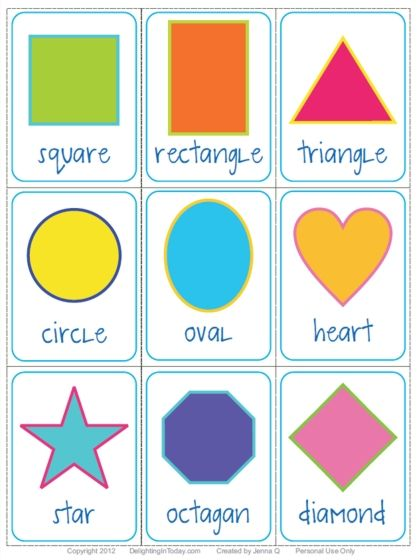
\includegraphics[height=.55\textheight]{images/samples/shapes_supervised}
					\caption*{Exemple de problème d'apprentissage supervisé: les classes (formes géométriques) sont données.}
				\end{figure}
			\end{frame}

			\begin{frame}{Apprentissage supervisé}
				Comment choisir ses attributs pour représenter chaque observation sous forme de vecteur?
				\begin{itemize}
					\item<2-> nombre de côtés;
					\item<3-> nombre de sommets;
					\item<4-> convexité;
					\item<5-> symmetrie par rotation;
					\item<6-> \dots;
				\end{itemize}
				\uncover<7->{
					Pour une observation, dont la forme (classe) est un carré, le vecteur d'attributs s'écrit:
					\[\begin{pmatrix}
						4\\
						4\\
						True\\
						False\\
						\vdots
					\end{pmatrix}\]
				}
			\end{frame}

			\begin{frame}{Apprentissage supervisé}
				\begin{figure}[H]
					\begin{center}
						\includestandalone[mode=buildnew, height=.5\textheight]{scatter_gender_dataset}
						\caption*{\tiny Exemple de problème de apprentissage supervisé: 2 attributs et 2 classes.}
					\end{center}
				\end{figure}
			\end{frame}

		\subsection{Formalisation}
			\begin{frame}{Fonction de décision}
				\begin{itemize}
					\item<1-> On suppose que ${\big((X^i, Y^i)\big)}_{i=1,\dots,n}$ sont des réalisations indépendantes et identiquement distribuées (i.i.d) de la loi $\mathbb{P}(X=x, Y=y) = p(x,y)$.
					\item<2-> On cherche une fonction de décision $D$ comme suit:
					\begin{align*}
						D: \mathbb{R}^d &\rightarrow \{1, \dots, C\} \\
						x &\mapsto D(x)
					\end{align*}
					\item<3-> On définit le \textbf{regret}, ou \textbf{risque}, d'une fonction de décision $D$ par:
					\begin{equation}
						R(D) \triangleq \mathbb{E}_{X,Y}(\mathbb{1}(D(X)\neq Y))
					\end{equation}
					\item<4-> Cette fonction calcule la mesure de l'espace d'attributs où $D(x) \neq y$:
					\begin{align*}
						R(D) &= \mathbb{P}(\{D(X)\neq Y\})\\
							&= \sum_{y = 1, \dots, C} \int_{x \in \mathbb{R}^d} \mathbb{1}(D(x)\neq y) p(dx, y)
					\end{align*}
				\end{itemize}
			\end{frame}
			\begin{frame}{Regret: mesure d'erreur}
				\begin{center}
					\begin{figure}[H]
						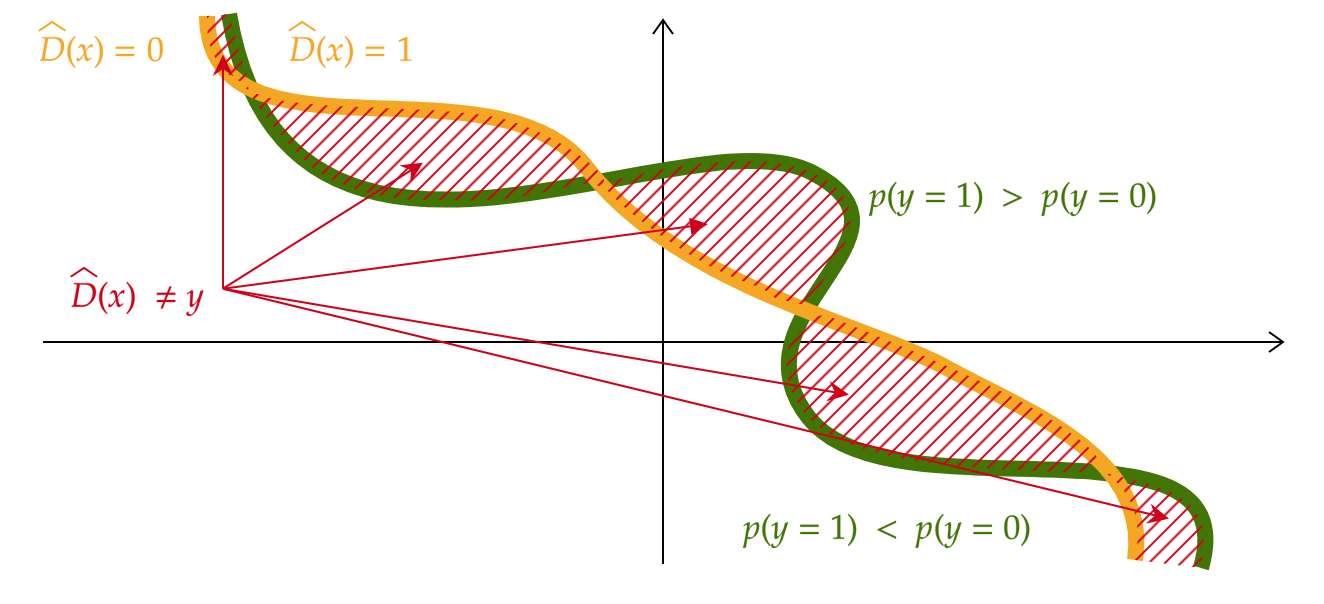
\includegraphics[width=.8\textwidth]{images/samples/illustration_difference_separator.png}
						\caption*{Illustration de l'espace \(D(X)\neq Y\): où \(Y \in \{0, 1\}\) et \(X \in \mathbb{R}^2\). Le regret est interprété comme l'\textbf{aire} de la surface hachurée selon la mesure \(p(dx, y)\)}
					\end{figure}	
				\end{center}
			\end{frame}
			\begin{frame}{Risque empirique}
				\begin{itemize}
					\item<1-> Le risque empirique est défini par:
						\begin{equation}
							R_n(D) \triangleq \frac{1}{n} . \sum_{i=1}^n \mathbb{1}_{D(X^i) \neq Y^i} \underset{n\infty}{\longrightarrow} R(D)
						\end{equation}
					\item<2-> Soit \(D^*_\mathscr{F}\) la fonction de décision optimale. Elle vérifie:
						\begin{equation}
							D^*_\mathscr{F} \triangleq \arg\min_{D \in \mathscr{F}} R(D)
						\end{equation}
					\item<3-> Soit \(\widehat D_n \) la fonction de décision empirique optimale:
						\begin{equation}
							\widehat D_n \triangleq \arg\min_{D \in \mathscr{F}} R_n(D)
						\end{equation}
					\item<3-> Exemple d'ensemble de recherche: 
					\begin{itemize}
						\item<4-> \(\mathscr{F}_{Total} \triangleq \{1, \dots, C\}^{\mathbb{R}^d}\): l'ensemble de toutes les fonctions possibles;
						\item<5-> \(\mathscr{F}_{Linear}\): l'ensemble de toutes les fonctions de séparation linéaires;
						\item<5-> \(\mathscr{F}_{Circle}\): l'ensemble de toutes les fonctions de séparation circulaires;
						\item<6-> \dots
					\end{itemize}
				\end{itemize}
			\end{frame}
			\begin{frame}{Choix de l'ensemble de recherche}
				\begin{itemize}
					\item<1-> Le choix de modèle de fonction de décision est important.
					\item<2-> Un choix naïf est de prendre toute les fonctions possibles. 
					\item<3-> Ce choix est mal adapté: on défini \(D_{naive}: x \mapsto \sum_{i=1,\dots,n} Y^i . \delta_{X^i}(x) + \mathbb{1}_{x \notin \{X^i, \forall i=1,\dots,n\}}\).
					\item<4-> On observe que: \(R_n(D_{naive}) = 0\). Il ne fait aucune erreur sur les données d'entraînement mais n'a aucun pouvoir de généralisation.
				\end{itemize}
			\end{frame}
			\begin{frame}{Décomposition biais/variance}
				\begin{itemize}
					\item<1-> On quantifie la différence de \(\widehat D_n \) par rapport à la fonction de décision optimale par~\cite{tsybakovpoly}:
						\begin{equation}
							R(\widehat D_n) - \min_{D \in \mathscr{F}_{Total}} R(D) = \overbrace{R(\widehat D_n) - R(D^*_\mathscr{F})}^{la\ variance} + \overbrace{R(D^*_\mathscr{F}) - \min_{D \in \mathscr{F}_{Total}} R(D)}^{le\ biais}
						\end{equation}
					\item<2-> Le terme de variance exprime la différence, purement stochastique, entre l'optimum \(D^*_\mathscr{F}\) sur l'ensemble  de recherche \(\mathscr{F}\) et l'optimum empirique;
					\item<3-> le terme de biais exprime la différence entre l'optimum \(D^*_\mathscr{F}\) par rapport à la vérité terrain.
				\end{itemize}
			\end{frame}
			\begin{frame}{Compromis biais/variance}
				\begin{itemize}
					\item<1-> La variance exprime l'\textit{erreur de paramètrage} entre la fonction de décision choisie \(\widehat D_n\) est la meilleure estimation possible \(D^*_\mathscr{F}\): sous \textit{certaines conditions}~\cite{tsybakovpoly}, il est prouvable que \(\widehat D_n \underset{n\infty}{\longrightarrow} D^*_\mathscr{F}\).
					\item<2-> Le biais exprime l'\textit{erreur de modélisation} entre le choix de type de fonction de décision et la vérité terrain. En pratique, on ne connaît pas la distribution réelle des données: il n'y a donc aucune garantie sur ce terme.
					\item<3-> Généralement, il y a un compromis à faire entre faible biais (overfitting) et faible variance (modèle peu compliqué \(\Rightarrow\) underfitting)~\cite{tsybakovpoly}.
				\end{itemize}
			\end{frame}
			\begin{frame}[plain]{Sur/Sous apprentissage: le compromis}
				\begin{figure}[H]
					\begin{center}
						\includestandalone[mode=buildnew, width=.7\textwidth]{scatter_separators}
						\vspace{-1em}
						\caption*{Illustration des cas de sur/sous apprentissage: $\mathscr{S}_1$ compromis de séparation, $\mathscr{S}_2$ surapprentissage et $\mathscr{S}_3$ sousapprentissage.}	
					\end{center}
				\end{figure}
			\end{frame}
			\begin{frame}{Discriminatif vs Génératif}
				\begin{itemize}
					\item<1-> On sait modéliser la distribution des classes $p(y)$ et celle des instances selon la classe $p(x\vert y)$ $\Longrightarrow$ méthode générative,
						\begin{itemize}
							\item<2-> Exemple: On s'intéresse à la détection de sexe selon deux mesures: taille et poids.
							\item<3-> On suppose que la répartition des sexes est équilibrée dans le monde $p(y=1) = p(y=0) = \frac{1}{2}$;
							\item<4-> Les répartitions des mesures selon les classes suivent des lois gaussiennes $X\vert Y=y \sim \mathscr{N}(m_y, \sigma_y)$.
						\end{itemize}
					\item<5-> On n'a aucune connaissance \textit{a priori}. On cherche à apprendre un modèle de $p(y \vert x)$ $\Longrightarrow$ méthode discriminative.
				\end{itemize}
			\end{frame}
		\subsection{Méthodes génératives}
			\begin{frame}{Règle de Bayes}
				\begin{equation}
					p(y \vert x) = \frac{p(x \vert y).p(y)}{p(x)}
				\end{equation}
				\begin{itemize}
					\item $p(y)$ : probabilité d'appartenir à la classe $y$.
					\item $p(x)$ : probabilité que l'attribut $X=x$.
					\item $p(x \vert y)$  : probabilité que la réalisation de $X$ soit $x$, sachant qu'il est dans la classe $y$.
					\item $p(y \vert x)$  : probabilité que la classe est $y$, sachant que la réalisation de $X$ est $x$.
				\end{itemize}
			\end{frame}
			\begin{frame}{La classe estimée}
				\begin{itemize}
					\item<1-> La classe estimée \(D(x)\) est la classe la plus probable sachant $X=x$: 
						\begin{equation}
							D(x) = \arg \max_{y=1,\dots,C} p(y \vert x)
						\end{equation}
					\item<2-> Dans le cas génératif, on a donc:
						\begin{align}
							D(x) &= \arg \max_{y=1,\dots,C} \frac{p(x \vert y).p(y)}{p(x)}\\
							D(x) &= \arg \max_{y=1,\dots,C} p(x \vert y).p(y)
						\end{align}
				\end{itemize}
			\end{frame}
			\begin{frame}{Exemple: Tennis or no Tennis}
				\begin{table}[H]
					\begin{center}
						\begin{tabular}{c c c c c}
							\toprule
							Temps (C) & Température (T) & Humidité (H) & Vent (V) & Tennis\\
							\midrule
							soleil & chaud & élevée & non & non\\
							soleil & chaud & élevée & oui & non\\
							couvert & chaud & élevée & non & oui\\
							pluie & tiède & élevée & non & oui\\
							pluie & froid & normale & non & oui\\
							pluie & froid & normale & oui & non\\
							couvert & froid & normale & oui & oui\\
							soleil & tiède & élevée & non & non\\
							soleil & froid & normale & non & oui\\
							pluie & tiède & normale & non & oui\\
							soleil & tiède & normale & oui & oui\\
							couvert & tiède & élevée & oui & oui\\
							couvert & chaud & normale & non & oui\\
							\bottomrule
						\end{tabular}
					\end{center}
				\end{table}
			\end{frame}
			\begin{frame}{Exemple: Tennis or no Tennis}
				\begin{itemize}
					\item \(p(Tennis = oui) = \frac{9}{14}\) et \(p(Tennis = non) = \frac{5}{14}\);
					\item On suppose que les différentes mesures de climats sont indépendantes \(P((C, T, H, V) \vert Tennis) = P(C\vert Tennis).P(T\vert Tennis).P(H\vert Tennis).P(V\vert Tennis)\);
					\item Application numérique pour \(X=(pluie, chaud,\)\textit{élevée}\(, non)\): 
						\[p(Tennis = oui \vert X) = p(X\vert Tennis = oui) . p(Tennis = oui) \approx 0.010582\]
						\[p(Tennis = non \vert X) = p(X\vert Tennis = non) . p(Tennis = non) \approx \boldmath 0.018286\]
						Donc quand quand il pleut, qu'il fait chaud, que la température est élevée et il n'y a pas de vent, on ne joue pas.
				\end{itemize}
			\end{frame}
		\subsection{Méthodes discriminatives}
			\subsubsection{Approches géométriques}
				\begin{frame}{Méthodes de centroïdes}
					\begin{itemize}
						\item<1-> On s'inspire du clustering: On assigne la classe dont le centroïde est le plus proche.
						\item<2-> On pose \(\mu_k = \frac{1}{\vert \{i\in\{1,\dots,n\}: Y^i = k\} \vert}.\sum_{\substack{i=1,\dots,n\\Y^i = k}} X^i\). On peut écrire:
							\begin{equation}
								D_{centroid}(x) \triangleq \arg \min_{k=1,\dots,C} \lVert x - \mu_k \rVert
							\end{equation}
					\end{itemize}
				\end{frame}
				\begin{frame}{Méthodes des centroïdes}
					\begin{figure}[H]
						\includestandalone[mode=buildnew, height=.5\textheight]{scatter_circles_class}
						\caption*{Problème de la méthode de centroïde: les deux classes sont cocentriques.}
					\end{figure}
				\end{frame}
				\begin{frame}{k-NN}
					\begin{itemize}
						\item<1-> On choisit les \(k\) instances les plus proches de l'observation \(x\). On assigne à cette observation la classe majoritaire parmi les \(k\) classes de ces voisins.
						\item<2-> Soit \(o_1,\dots,o_n\) les indices qui guarantissent: \(\lVert x - X^{o_1} \rVert \leq \lVert x - X^{o_2} \rVert \dots \leq \lVert x - X^{o_n} \rVert\). Les \(k\) plus proches voisins sont donc \(\{X^{o_1}, X^{o_2},\dots,X^{o_k}\}\).
						\item<3-> On définit donc la fonction de décision du k-NN par:
							\begin{equation}
								D_{knn}(x) \triangleq \arg \max_{c=1,\dots,C} \sum_{i=1,\dots,k} \mathbb{1}_{Y^{o_i} = c}
							\end{equation}
						\item<4-> Plus k augmente, plus les frontières seront lisses.
					\end{itemize}
				\end{frame}

			\subsubsection{Arbre aléatoire}
				\begin{frame}{Arbres de décision: exemple}
					\begin{figure}[H]
						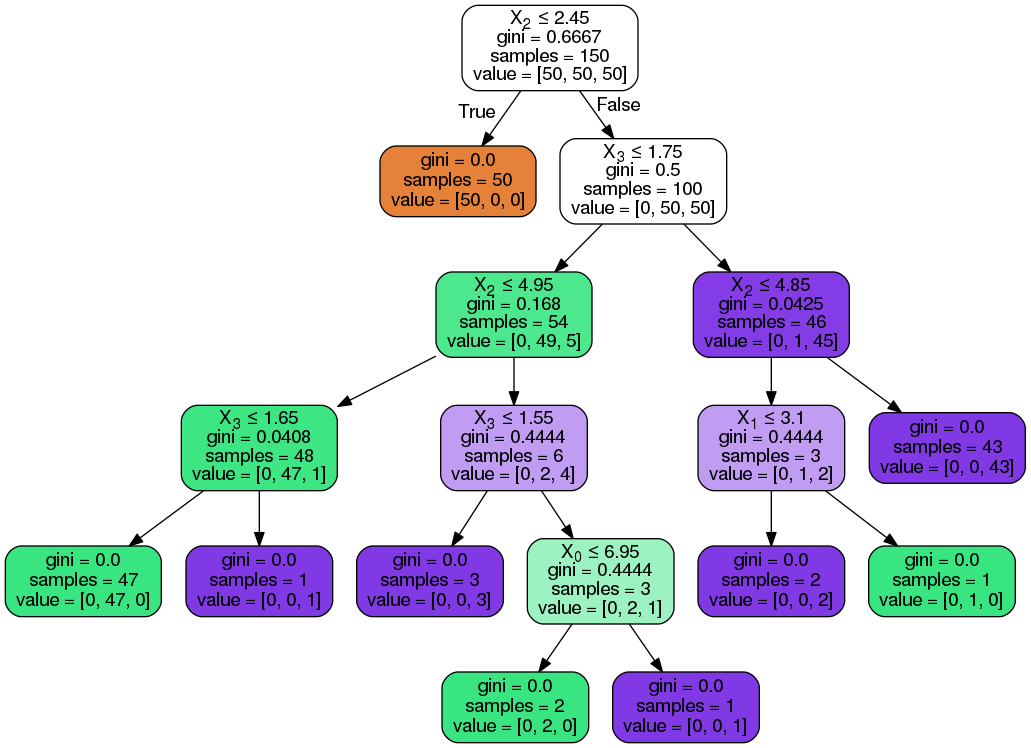
\includegraphics[width=.65\textwidth]{images/samples/example_dt_iris_dataset.png}
						\caption*{Exemple d'arbre de décision appliquée à le jeu de données Iris: 4 attributs (longueur de sépale, largeur de sépale, longueur de pétale et largeur de pétale) et 3 classes: (``Iris Setosa'', ``Iris Versicolour'', ``Iris Virginica'').}
					\end{figure}
				\end{frame}
				\begin{frame}{Arbres de décision: construction}
					\begin{itemize}
						\item<1-> On commence par la racine: toutes les instances sont présentes.
						\item<2-> On choisit l'attribut et le seuil qui permettent de séparer le mieux les observations en groupes homogènes.
						\item<3-> On répète la deuxième étape à chaque groupe jusqu'à:
							\begin{itemize}
								\item<4-> Atteindre un groupe pur: il ne contient que des observations ayant la même classe;
								\item<5-> Atteindre un critère d'arrêt.
							\end{itemize}
					\end{itemize}
				\end{frame}
				\begin{frame}{Arbres de décision: critère d'arrêt}
					Exemples:
					\begin{itemize}
						\item<1-> Nombre minimum d’observations par groupe.
						\item<2-> Toutes les observations d’une branche sont de la même classe (feuille pure).
						\item<3-> Degré de pureté maximal atteint \(p\): \(\frac{\vert Y \vert}{\vert G\vert} \geq p\), où: \(Y\) est l'ensemble des instances de la classe majoritaire et \(G\) l'ensemble de toutes les observations dans le groupe en question. Le cas précédent est un cas particulier avec \(p = 1\).
						\item<4-> Profondeur\footnote{le nombre maximal de choix pour aller du jeu de données initial à une feuille} de l’arbre maximale atteinte.
					\end{itemize}
				\end{frame}
				\begin{frame}{Arbres de décision: mesure d'hétérogénéité}
					\begin{itemize}
						\item<1-> Soit \(S\) une famille (répétitivité possible) d'éléments. Dans notre cas, \(S := ((Y^i)_{i=1,\dots,n})\).
						\item<2-> On définit \(p_k := \frac{\vert \big\{i \in \{1,\dots,n\}: Y^i = k\big\}\vert}{n}\) la probabilité empirique de la valeur \(k \in \{1,\dots,C\}\).
						\item<3-> On désire mesurer son hétérogénéité par rapport aux classes \(Y^i\). Soit \(H: S\mapsto H(S)\) une telle mesure.
						\item<4-> Le cas le moins hétérogène est le cas \(\exists k_0, \forall k, p_k = \delta_{k_0}(k)\). Dans ce cas, \(H(S)\) doit atteindre son minimum.
						\item<5-> Le maximum de \(H\), par contre, est atteint dans le cas où toutes les valeurs de classes sont également probables: \(p_k = \frac{1}{C}, \quad \forall k=1,\dots,C\): le cas le plus hétérogène.
						\item<6-> Exemples de telles mesures:
							\begin{itemize}
								\item L'entropie:
									\begin{equation}
										H_E \triangleq - \sum_{k=1}^C p_k . \ln(p_k)
									\end{equation}
								\item L'indice de Ginni:
									\begin{equation}
										H_G \triangleq \sum_{k=1}^C p_k(1-p_k) = 1 - \sum_{k=1}^C p_k^2
									\end{equation}
							\end{itemize}
					\end{itemize}
				\end{frame}
				\begin{frame}{Arbres de décision: mesure de qualité de séparation}
					\begin{itemize}
						\item<1-> Soit \(\big(S_k\big)_{k = 1, \dots, K}\) une \(K\)-partition de \(S\).
						\item<2-> Une bonne séparation se traduit par un gain d'homogéniété après séparation: i.e. les sous-ensembles \(S_k\) sont moins hétérogènes que l'ensemble d'origine.
						\item<3-> On définit le gain de la partition \(\big(S_k\big)_{k = 1, \dots, K}\) par:
							\begin{equation}
								G\big((S_1, \dots, S_K)\big) \triangleq H(S) - \sum_{k=1}^K \frac{\vert S_k \vert}{\vert S \vert}H(S_k)
							\end{equation}
						\item<4-> Trois cas se précisent:
							\begin{itemize}
								\item<5-> \(G\big((S_1, \dots, S_K)\big) > 0\): la partition permet de bien séparer \(S\) de façon à avoir des sous-ensembles plus ``purs'';
								\item<6-> \(G\big((S_1, \dots, S_K)\big) = 0\): la partition donne des sous-ensembles aussi hétérogène que \(S\): on ne gagne rien;
								\item<7-> \(G\big((S_1, \dots, S_K)\big) < 0\): la partition perd en ``pureté'' par rapport à \(S\).
							\end{itemize}
					\end{itemize}
				\end{frame}
				\begin{frame}{Arbres de décision: mesure de qualité de séparation}
					\begin{itemize}
						\item<1-> L'arbre naïf choisirait des critères sur \(Y^i\). Sauf que ces classes ne seront pas observables, en phase, de test.
						\item<2-> On choisit le couple attribut \(X_c\) et seuil \(s\) le plus discriminant: les seules partitions possibles sont: \(S_1 := \{i \in S: X_c - s > 0\}\) ou \(S_2 := \{i \in S: X_c - s \leq 0\}\).
						\item<3-> Dans ce cas, par abus de language, on note le gain de cette séparation: \(G(c, s) := G\big((S_1, S_2)\big)\)
						\item<4-> Cela revient à résoudre le problème:
							\begin{equation}
								\arg \max_{\substack{c=1,\dots,d\\s \in \mathscr{S}_c}} G(c, s)
							\end{equation}
							où \(\mathscr{S}_c\) est l'ensemble de valeurs possibles pour l'attribut \(c\).
					\end{itemize}
				\end{frame}
				\begin{frame}{Exemple: Tennis or no Tennis}
					\begin{table}[H]
						\begin{center}
							\begin{tabular}{c c c c c}
								\toprule
								Temps (C) & Température (T) & Humidité (H) & Vent (V) & Tennis\\
								\midrule
								soleil & chaud & élevée & non & non\\
								soleil & chaud & élevée & oui & non\\
								couvert & chaud & élevée & non & oui\\
								pluie & tiède & élevée & non & oui\\
								pluie & froid & normale & non & oui\\
								pluie & froid & normale & oui & non\\
								couvert & froid & normale & oui & oui\\
								soleil & tiède & élevée & non & non\\
								soleil & froid & normale & non & oui\\
								pluie & tiède & normale & non & oui\\
								soleil & tiède & normale & oui & oui\\
								couvert & tiède & élevée & oui & oui\\
								couvert & chaud & normale & non & oui\\
								\bottomrule
							\end{tabular}
						\end{center}
					\end{table}
				\end{frame}
				\begin{frame}{Exemple: Tennis or no Tennis}
					\begin{itemize}
						\item<1-> Racine: 9 | 4 \(\longrightarrow H_G = 1 - \frac{1}{9} - \frac{4}{9} = \frac{4}{9}\) ;
							\begin{itemize}
								\small
								\item c=C, s=couvert: \(\longrightarrow H_G (C > s) = 1 - \frac{9}{25} - \frac{4}{25} = \frac{12}{25}\) and \(H_G (C \leq s) = 1- \frac{25}{49} - \frac{4}{49} = \frac{20}{49}\).
									\(G(C, couvert) = \frac{4}{9} - \frac{1}{5} . \frac{12}{25} - \frac{1}{7} . \frac{12}{49} \approx 0.2901\)
								\item c=C, s=pluie \(\longrightarrow H_G (C > s) = 1 - \frac{25}{64} - \frac{9}{64} = \frac{15}{32}\) and \(H_G (C \leq s) = 1- \frac{1}{16} - \frac{9}{16} = \frac{3}{8}\).
									\(G(C, couvert) = \frac{4}{9} - \frac{1}{4} . \frac{3}{8} - \frac{1}{8} . \frac{15}{32} \approx 0.2921\)
								\item c=T, s=tiède \(\longrightarrow H_G (C > s) = 1 - \frac{1}{4} - \frac{1}{4} = \frac{1}{2}\) and \(H_G (C \leq s) = 1- \frac{36}{64} - \frac{4}{64} = \frac{3}{8}\).
									\(G(C, couvert) = \frac{4}{9} - \frac{1}{2} . \frac{1}{2} - \frac{1}{8} . \frac{3}{8} \approx 0.1476\)
								\item c=T, s=froid \(\longrightarrow H_G (C > s) = 1 - \frac{25}{64} - \frac{9}{64} = \frac{15}{32}\) and \(H_G (C \leq s) = 1- \frac{1}{16} - \frac{9}{16} = \frac{3}{8}\).
									\(G(C, couvert) = \frac{4}{9} - \frac{1}{4} . \frac{3}{8} - \frac{1}{8} . \frac{15}{32} \approx 0.2921\)
								\item \textbf{c=H, s=normale} \(\longrightarrow H_G (C > s) = 1 - \frac{1}{4} - \frac{1}{4} = \frac{1}{2}\) and \(H_G (C \leq s) = 1- \frac{25}{36} - \frac{1}{36} = \frac{5}{18}\).
									\(G(C, couvert) = \frac{4}{9} - \frac{1}{6} . \frac{1}{2} - \frac{1}{6} . \frac{5}{18} \approx 0.314814\)
								\item c=V, s=non \(\longrightarrow H_G (C > s) = 1 - \frac{9}{25} - \frac{4}{25} = \frac{12}{25}\) and \(H_G (C \leq s) = 1- \frac{25}{49} - \frac{4}{49} = \frac{20}{49}\).
									\(G(C, couvert) = \frac{4}{9} - \frac{1}{5} . \frac{12}{25} - \frac{1}{7} . \frac{20}{49} \approx 0.2901\)
							\end{itemize}
					\end{itemize}
				\end{frame}
				\begin{frame}{Exemple: 2D}
					\begin{figure}[H]
						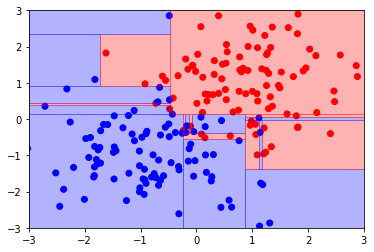
\includegraphics[width=.7\textwidth]{images/samples/boundary_decision_tree.png}
						\caption*{Visualization de la frontière de l'arbre de décision avec 2 attributs. Plus l'arbre est profond, plus la frontière est accidentée.}
					\end{figure}
				\end{frame}

			\subsubsection{Forêt aléatoire}
				\begin{frame}{Méthodes ensemblistes}
					\begin{figure}[H]
						\includestandalone[mode=buildnew, height=.5\textheight]{ensemblist_method}
						\caption*{Principe des méthodes ensemblistes: chaque fonction de décision (classifieur) a une région où il est mauvais. Une bonne méthode ensembliste cherchera, pour chaque point de l'espace, à éviter d'utiliser les classifieurs qui donnent de mauvais résultats en choisissant la meilleure combinaison de classifieurs.}
					\end{figure}
				\end{frame}
				\begin{frame}{Méthodes ensemblistes: forêt aléatoire}
					\begin{figure}[H]
						\includestandalone[mode=buildnew, height=.6\textheight]{circles_dt}
						\caption*{Frontière d'un arbre de décision: on remarque qu'il sur-apprend sur les observations données.}
					\end{figure}
				\end{frame}
				\begin{frame}{Méthodes ensemblistes: forêt aléatoire}
					\begin{figure}[H]
						\includestandalone[mode=buildnew, height=.6\textheight]{circles_rf}
						\caption*{Frontière d'une forêt aléatoire: on multiplie les arbres de décisions (toute les couleurs sauf le violet) peu profonds (donc qui sous-apprennent). Chaque arbre donne la classe probable selon lui. Elles sont toutes conbinées pour donner la classe finale: séparation en violet.}
					\end{figure}
				\end{frame}
				\begin{frame}{Forêt aléatoire: construction}
					\begin{itemize}
						\item<1-> Pour construire une forêt aléatoire qui contient \(A\) arbres;
						\item<2-> Pour chacun des \(A\) arbres, on sélectionne aléatoirement une sous partie des attributs: \(X^i_{(a)} = \begin{pmatrix}
							X^i_{o^a_1} & X^i_{o^a_2} & \dots & X^i_{o^a_{d_a}}
						\end{pmatrix}^T, \quad \forall a = 1,\dots,A  i=1,\dots,n\).
						\item<3-> Chaque arbre de décision sera construit en fonction d'un sous-ensemble des données initiales et dans un sous-espace de l'espace d'attributs.
						\item<4-> Pour connaître la classe de \(x \in \mathbb{R}^d\), on sélectionne les attributs \(x_a, \quad \forall a = 1,\dots,A\) et on fait passer chacun par l'arbre qui correspond.
						\item<5-> Cela donne les classes \(y_a, \quad \forall a = 1,\dots,A\). Par vote majoritaire, on décide la classe la plus probable:
							\begin{equation}
								D_{random\ forest, absolute} (x) \triangleq \arg \max_{k=1,\dots,C} \vert \{a \in \{1,\dots,A\}: y_a = k\} \vert
							\end{equation}
						\item<6-> On peut extraire aussi le couple (classe, probabilité) de chaque arbre \((y_a, p_a), \quad \forall a = 1,\dots,A\). On relache la définition précédente pour donner:
							\begin{equation}
								D_{random\ forest, weighted} (x) \triangleq \arg \max_{k=1,\dots,C} \sum_{a=1}^{A} p_a(y_a = k)
							\end{equation}
					\end{itemize}
				\end{frame}
	
	\section{Evaluation de classifieur}
		\subsection{Principe}
			\begin{frame}{Evaluer une classification}
				\begin{itemize}
					\item<1-> Évaluation: comparaison de résultats d’une classification aux données de référence.
					\item<2-> On compte le nombre de fois où le classifieur donne une mauvaise réponse, à opposer au nombre de fois où il donne une bonne réponse.
					\item<3-> Plus la vérité terrain est exhaustive (couvre de classes d’intérêt), meilleure est la compréhension des limites de la classification.
				\end{itemize}
			\end{frame}
			\begin{frame}{Motivation}
				\begin{itemize}
					\item<1-> Comparaison de classifieur : i.e. décision pour savoir si un classifieur est meilleur qu’un autre;
					\item<2-> Choisir les meilleurs paramètres pour un modèle de classifieur.
				\end{itemize}
			\end{frame}
		\subsection{Matrice de confusion et ratios}
			\begin{frame}{Matrice de confusion}
				\begin{table}[H]
					\begin{tabular}{| c | c | c | c | c | c |}
						\hline
						& \multicolumn{5}{c |}{Vérité terrain}\\
						\hline
						\multirow{5}{*}{\rotatebox{90}{Prédictions}}& & 1 & 2 & \dots & C\\
						\cline{2-6}
						& 1 & \(n_{11}\) & \(n_{12}\) & & \(n_{1C}\)\\
						\cline{2-6}
						& 2 & \(n_{21}\) & \(n_{22}\) & & \(n_{2C}\)\\
						\cline{2-6}
						& \rotatebox{90}{\dots} & & & & \\
						\cline{2-6}
						& C & \(n_{C1}\) & \(n_{C2}\) & & \(n_{CC}\)\\
						\hline
					\end{tabular}
					\caption*{Matrice de confusion: \(n_{ij}\) nombre d'éléments de classe \(j\) et prédits de classe \(i\).}
				\end{table}
			\end{frame}
			\begin{frame}{Ratios: rappel et précision}
				\begin{itemize}
					\item<1-> Rappel: exhaustivité de la détection. Parmi les éléments qui font partie d'une classe donnée, combien sont bien prédit correctement:
						\begin{equation}
							R = \frac{n_{jj}}{\underbrace{\sum_{i=1}^C n_{ij}}_{\text{vérité terrain de classe } j}}
						\end{equation}
					\item<2-> Précision: exactitude des prédiction. Parmi les éléments qui sont prédits être d'une classe donnée, combien en font partie réellement:
						\begin{equation}
							P = \frac{n_{ii}}{\underbrace{\sum_{j=1}^C n_{ij}}_{\text{éléments prédits de classe } i}}
						\end{equation}
				\end{itemize}
			\end{frame}
			\begin{frame}{Ratios: F-score et bonne classification}
				\begin{itemize}
					\item<1-> F-score: moyenne harmonique de la précision et du rappelle:
						\begin{equation}
							F_{score} = \frac{2}{\frac{1}{P} + \frac{1}{R}}
						\end{equation}
					\item<2-> Taux de bonne classification:
						\begin{equation}
							OA = \frac{\sum_{i=1}^C n_{ii}}{\sum_{i,j=1}^C n_{ij}}
						\end{equation}
				\end{itemize}
			\end{frame}
			\begin{frame}{Receiver operating characteristic}
				Dans le case de classification binaire, on calcule les deux ratios:
				\begin{itemize}
					\item<1-> Taux de Faux Positifs (FPR):
						\begin{equation}
							FPR = \frac{n_{00}}{n_{00} + n_{10}}
						\end{equation}
					\item<2-> Taux de Vrais Positifs (TPR):
						\begin{equation}
							TPR = R
						\end{equation}
				\end{itemize}
				\uncover<3->{
					On affiche donc le TPR en fonction du FPR: on l'appelle l'espace Receiver Operating Characteristic (ROC).
				}
			\end{frame}
			\begin{frame}{Espace ROC}
				\begin{figure}[H]
					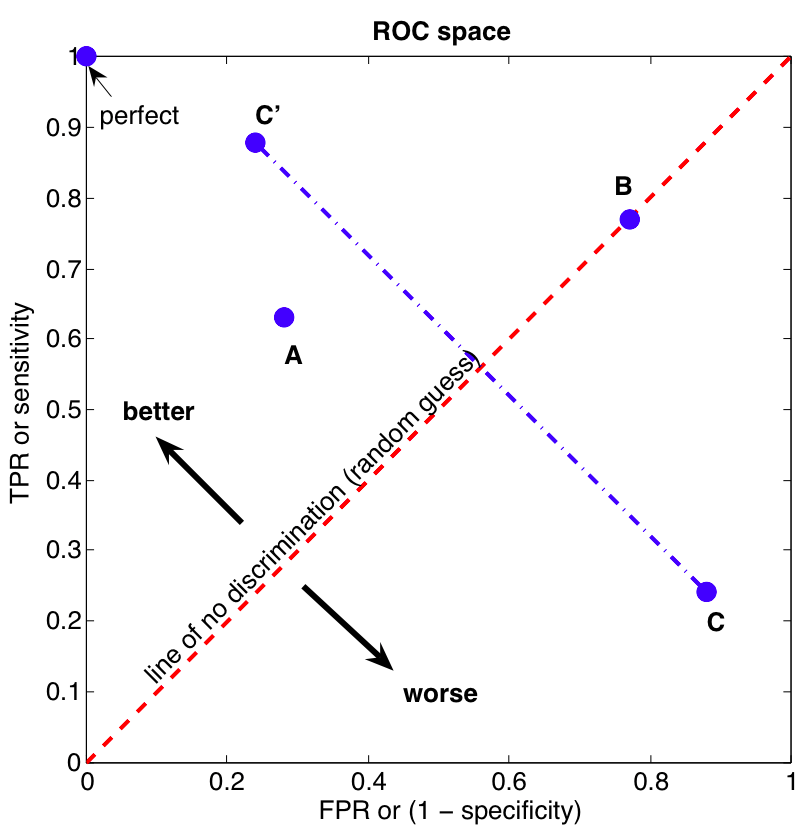
\includegraphics[width=.45\textwidth]{images/samples/roc.png}
					\caption*{Espace de ROC~\cite{schrynemackers2009using}. Le classifieur correspondant au point (C) ``dés-apprend'': il est pire que le classifieur aléatoire.}
				\end{figure}
			\end{frame}
			\begin{frame}{Courbe ROC}
				\begin{itemize}
					\item<1-> Un classifieur discret produit un unique couple (FPR, TPR), qui correspond à un point unique dans l’espace ROC.
					\item<2-> Certains classifieurs fournissent un score ou une probabilité d’appartenance: le degré de confiance en l’appartenance à la classe.
					\item<3-> On peut évaluer la qualité d'une classification en fonction d'un ensemble de seuils du score obtenu en sortie. Chaque seuil crée un point différent dans l'espace ROC.
					\item<4-> On obtient ainsi une courbe ROC pour chaque seuil envisageable.
				\end{itemize}
			\end{frame}
			\begin{frame}{Courbes ROC}
				\begin{figure}[H]
					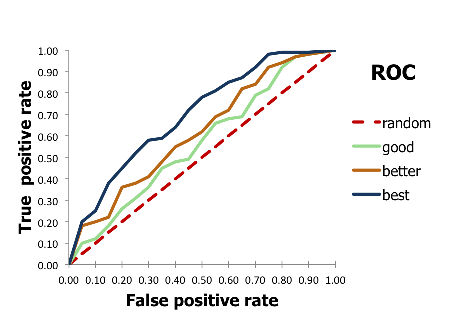
\includegraphics[width=.6\textwidth]{images/samples/roc_curves.png}
					\caption*{Exemples de courbes ROC~\cite{ROCS}.}
				\end{figure}
			\end{frame}
			\begin{frame}{Area Under Curve}
				\begin{itemize}
					\item<1-> On peut définir un seul scalaire pour ordonner les courbes ROC. On définit l'aire sous la courbe (Area Under Curve) d'un classifieur \(\mathscr{C}\) avec une courbe \(\mathscr{R}(\mathscr{C})\):
					\begin{equation}
						AUC(\mathscr{C}) \triangleq \int_{FPR\in[0,1]} \mathscr{C}(FPR)
					\end{equation}
					\item<2-> Plus le \(AUC\) est grand, meilleur est le classifieur.
					\item<3-> Le classifieur aléatoire a \(AUC(Rand) = 0.5\).
					\item<4->\(AUC(\mathscr{C}) \leq 0.5 \Longrightarrow\) \(\mathscr{C}\) apprend mal.
				\end{itemize}
			\end{frame}
		\subsection{Validation croisée}
			\begin{frame}{Principe}
				\begin{itemize}
					\item<1-> Les échantillons jouent un rôle important dans l'apprentissage.
					\item<2-> Comment réagissent les scores d'évaluation d'un classifieur quand on rajoutte plus de données?
					\item<3-> Comment choisir les meilleures paramètres d'un classifieur pour avoir les résultats les plus stables possibles?
				\end{itemize}
			\end{frame}
			\begin{frame}{Procédure}
				\begin{itemize}
					\item<1-> On divise donc la base de données en \(k\) parties.
					\item<2-> On fusionne \(k-1\) parties et entraîne dessus le classifieur. On teste sur la partie restante.
					\item<3-> Il y a donc \(\binom{k}{k-1} = k\) cas.
					\item<4-> On conduit les \(k\) expériences. On peut donc calculer des statistiques sur ces résultats.
					\item<5-> On peut ainsi comparer des classifieurs en comparant ces statistiques.
				\end{itemize}
			\end{frame}
	\section{Références}
	\begin{frame}[allowframebreaks]{Références}
		\bibliographystyle{apalike}
		\bibliography{references.bib}
	\end{frame}

\end{document}
